\documentclass[a4paper,10pt]{article}
%%%%%%%%%%% Package %%%%%%%%%%%
\usepackage{amssymb}  % Used for math symbols.
\usepackage{amsmath}  % Used for math environments.
\usepackage[french,english]{babel} % Used to define the language.
\usepackage{datetime} % Used for the dynamic date.
\usepackage{float}    % Used to force figure to stay on place with [H]
\usepackage[T1]{fontenc} % Used to display french character correctly.
\usepackage{geometry} % Used to change margin.
\usepackage{graphicx} % Used to display image/graphic.
\usepackage{hyperref} % Used for hypertext.
\usepackage{inputenc} % Used to specify encodage.
\usepackage{listings} % Used to display code.
\usepackage{lipsum}   % Used to generate lorem ipsum
\usepackage{setspace} % Used to define space between lines.
\usepackage{tabularx} % Used for some table

%%%%%%%%%%% Param %%%%%%%%%%%
\geometry{top=2.4cm, bottom=2.4cm, left=2.4cm , right=2.4cm}
\hypersetup{
    colorlinks=true,            % Color link instead of framing links.
    linkcolor=blue,             % Color of intern link.
    urlcolor=blue,              % Color of url link.
}
\inputencoding{utf8}            % Define the encoding as utf8.
\lstset{
  language={}, % Aucun langage spécifique
  basicstyle=\tt\footnotesize, % Police de caractères // \tt\footnotesize
  numbers=left, % Numérotation des lignes à gauche
  numberstyle=\tiny, % Style de numérotation des lignes // \tiny\color{mygray}
  frame=single, % Encadrement du code
  breaklines=true, % Saut de ligne automatique
  showstringspaces=false % Ne pas afficher les espaces dans les chaînes de caractères
}
\setlength{\parindent}{15pt}    % Define indentation size (default=15pt)
\setstretch{1}                  % Define space between lines (default=1)

%%%%%%%%%%% Useful link %%%%%%%%%%%
% https://www.tablesgenerator.com/ % Useful to create LaTeX table
 
%%%%%%%%%%% Commands %%%%%%%%%%%
\newcommand{\HRule}{\rule{\linewidth}{0.5mm}} % Print a line
\newcommand{\schoolyear}{\the\numexpr\year-(\ifnum\month<9 1\else 0\fi)\relax-\the\numexpr\year+(\ifnum\month<9 0\else 1\fi)} % Print the current academic year.

%%%%%%%%%%% Document %%%%%%%%%%%
\begin{document}

%%%%%%%%%%% Front page %%%%%%%%%%%
\begin{titlepage}
   \begin{center}

    % Upper part of the page. The '~' is needed because 
    % only works if a paragraph has started.
    ~\\[4cm]
    
\includegraphics[scale=0.9]{images/facsa.png}
    ~\\[1.5cm]
    % Title
    \HRule \\[0.4cm]
    {\huge Introduction to Machine Learning\\[0.4cm] }

    \HRule \\[1cm]
    
    \textsc{\Large Bias and variance analysis}\\[2cm]
    \vspace{2cm}
    % Author and supervisor
    \begin{minipage}{0.3\textwidth}
      \begin{flushleft} \large
        Arthur \textsc{GRAILLET}
        Robin \textsc{FONBONNE}
        Thomas \textsc{ROTHEUDT}
      \end{flushleft}
    \end{minipage}
    \begin{minipage}{0.3\textwidth}
      \begin{flushright}\large
        s182019
        s182200
        s191895
      \end{flushright}
    \end{minipage}

    \vfill

    % Bottom of the page
    {\large Academic year \schoolyear}

  \end{center}
\end{titlepage}
\newpage

%%%%%%%%%%% Report %%%%%%%%%%%

%%% Question 1: Analytical derivations
\section{Analytical derivations}
\begin{enumerate}
    %% Question 1.1: Show that the expected generalization error...
    \item 
    We have the expected generalization error of the k-Nearest Neighbours algorithm:
    $$
    E_{LS}\{E_{y\mid \textbf{x}}\{(y - \hat{y}(\textbf{x};LS,k))^2\}\}
    $$
    
    We can substitude $y$ by $f(\textbf{x}) + \epsilon$ and expand the square in the expected squared error written as
    $$
    E_{y\mid \textbf{x}}\{(y - \hat{y}(\textbf{x};LS,k))^2\}
    $$
    to obtain:
    $$
    E_{y\mid \textbf{x}}\{(f(\textbf{x}) - \hat{y}(\textbf{x};LS,k))^2 + 2\epsilon(f(\textbf{x})-\hat{y}(\textbf{x};LS,k)) + \epsilon^2\}
    $$

    Since $E[\epsilon] = 0$ and $\epsilon$ is independent of $f(x)$ and $\hat{y}(\textbf{x};LS,k)$ the cross-term vanishes and the formula becomes:
    $$
    E_{y\mid \textbf{x}}\{(y - \hat{y}(\textbf{x};LS,k))^2\} = (f(\textbf{x})-\hat{y}(\textbf{x};LS,k))^2 + E[\epsilon^2]
    $$

    Since $\epsilon \sim \mathcal{N}(0, \sigma^2)$, we have $E[\epsilon^2] = \sigma^2$ it can be written as:
    $$
    (f(\textbf{x})-\hat{y}(\textbf{x};LS,k))^2 + \sigma^2
    $$

    We can rewrite $\hat{y}(\textbf{x};LS,k)$ as the average of the function values at the k-nearest neighbors:
    $$
    \hat{y}(\textbf{x};LS, k) = \frac{1}{k}\sum^k_{l=1}y_{(l)}
    $$
    where $y_{(l)} = f(\textbf{x}_{(l)}) + \epsilon$ (with $\epsilon \sim \mathcal{N}(0, \sigma^2)$). Therefore it can be written as:
    $$
    \hat{y}(\textbf{x};LS, k) = \frac{1}{k}\sum^k_{l=1}f(\textbf{x}_{(l)}) + \epsilon = \frac{1}{k}\sum^k_{l=1}f(\textbf{x}_{(l)}) + \frac{1}{k}\sum^k_{l=1}\epsilon
    $$

    The expected squared error can be decomposed as follows:
    $$
    \sigma^2  
    + \left(f(\textbf{x})-\frac{1}{k}\sum^k_{l=1}f(\textbf{x}_{(l)})\right)^2
    + 2\left(f(\textbf{x})-\frac{1}{k}\sum^k_{l=1}f(\textbf{x}_{(l)})\right) \left(\frac{1}{k}\sum^k_{l=1}\epsilon\right)
    + \left(\frac{1}{k}\sum^k_{l=1}\epsilon\right)^2
    $$
    Since $\epsilon$ is an independent random variable with a mean of zero, the cross-term has an expectation of zero. We can write the expected generalization error as:
    $$
    E_{LS}\{E_{y\mid \textbf{x}}\{(y - \hat{y}(\textbf{x};LS,k))^2\}\} =
    E_{LS}\left(\sigma^2\right)
    + E_{LS}\left[\left(f(\textbf{x})-\frac{1}{k}\sum^k_{l=1}f(\textbf{x}_{(l)})\right)^2\right]
    + E_{LS}\left[\left(\frac{1}{k}\sum^k_{l=1}\epsilon\right)^2\right]
    $$

    The expectation of a constant is the constant itself and the expectation of the third term
    $$
    E_{LS}\left[\left(\frac{1}{k}\sum^k_{l=1}\epsilon\right)^2\right] = \frac{\sigma^2}{k}
    $$
    because $\text{Var}(\epsilon) = \sigma^2$.

    Since \textbf{x} is fixed, the second term is also fixed. Taking the expectation $E_{LS}$ over this term has no effect.

    Therefore we can conclude that
    $$
    E_{LS}\{E_{y\mid \textbf{x}}\{(y - \hat{y}(\textbf{x};LS,k))^2\}\} =
    \sigma^2
    + \left[f(\textbf{x})-\frac{1}{k}\sum^k_{l=1}f(\textbf{x}_{(l)})\right]^2
    + \frac{\sigma^2}{k}
    $$

    The first term represents the noise, the second the bias, and the third the variance. 

    %% Question 1.2: Let us now assume that the problem is unidimensional...
    \item 
    We know that $f(x) = x^2$. Since we have to evaluate the bias and variance at $x = 0$ we know that $f(x) = 0$.

    The bias can be written as:
    $$
    \text{bias} = \frac{-1}{k}\sum^k_{l=1}({x}_{(l)})^2
    $$
    Since the training inputs are symmetrically distributed around $x=0$ on a uniform grid in [-1,+1], the k-neighbors of $x=0$ include the point $x=0$, $k'$ positive points, and $k'$ negative points. We have that
    $$
    \sum^k_{l=1}({x}_{(l)})^2 = 2\sum^{k'}_{l=1}\left(\frac{i}{N'}\right)^2 = \frac{2}{(N')^2}\sum^{k'}_{l=1}i^2
    $$
    We can use the formula to write the sum as a function of $k'$:
    $$
    \frac{2}{(N')^2}\sum^{k'}_{l=1}i^2 = \frac{2}{(N')^2}\frac{k'(k'+1)(2k'+1)}{6}
    $$
    The result must be expressed as a function of k and N, we can replace $k'$ and $N'$ with the relation $k' = \frac{k-1}{2}$ and $N' = \frac{N-1}{2}$:
    $$
    \frac{2}{\frac{(N-1)^2}{4}}\frac{(\frac{k-1}{2})(\frac{k-1}{2}+1)(k-1+1)}{6} = \frac{k(k^2 - 1)}{3(N-1)^2}
    $$
    The bias can be written as a function of k and N:
    $$
    \text{bias} = \frac{-(k^2 - 1)}{3(N-1)^2} 
    $$


    The variance is already expressed as a function of $\sigma$ and $k$:
    $$
    \text{variance} = \frac{\sigma^2}{k}
    $$

    
    %% Question 1.3: Discuss the impact of N, k, an σ on bias and variance. Are there 
    % some surprising or missing dependences? If so, try and explain them.
    \item 
    \begin{itemize}
        \item 
        $k$ appears in the formula of the variance and it is obvious that a greater k leads to a smaller variance. But increasing $k$ may lead to an increase of the bias because we would consider more distant points which reduce the flexibility of the model.
        \item
        Increasing the size $N$ of the learning sample generally leads to a denser distribution, therefore with the same $k$ and $\sigma$, the k-nearest neighbors around $x$ will be closer to $x$ and we can expect that they better represent the local behavior of $f(x)$.
        We can say that larger N leads to smaller bias. If we consider the problem explain in 2, we can see that the size $N$ is in the bias formula and increasing $N$ reduces the bias.

        $N$ has no direct impact on the variance but we can note that a larger $N$ allows a larger $k$ which leads to a lower variance. 
        \item 
        A greater $\sigma$ means more noise and as we may expect it increases the variance but does not impact the bias.
    \end{itemize}


    
    %% Question 1.4: For all combinations of N in {25, 50} and σ ∈ {0.0, 0.1, 0.2}, determine 
    % the value k∗ of k that minimizes the expected generalization error at x = 0.
    \item
    As suggested we'll compute the minimum by running actual experiments. We have to minimize this function:
    $$
    f(k) = \sigma^2 + \left[\frac{-(k^2 - 1)}{3(N-1)^2}\right]^2 + \frac{\sigma^2}{k}
    $$
    By testing every possible value of $k$ such that $k = 2k' + 1$ with $0 \le k' \le \frac{N-1}{2}$ for each combination of $N$ and $\sigma$ we have the following results:
    \begin{table}[H]
      \centering
      \begin{tabular}{l|l|l|l|}
      \cline{2-4}
                               & $\sigma = 0$ & $\sigma = 0.1$ & $\sigma = 0.2$ \\ \hline
      \multicolumn{1}{|l|}{$N = 25$} & 1  &  5  &  7 \\ \hline
      \multicolumn{1}{|l|}{$N = 50$} & 1  &  11   &  13 \\ \hline
      \end{tabular}
      \caption{Table of $k^*$ considering only odd values for k}
    \end{table}
    The cells represent the $k^*$ for each combination.

    If we can still consider even values for $k$ with the formula obtained considering only odd values of $k$ we would have:
    \begin{table}[H]
      \centering
      \begin{tabular}{l|l|l|l|}
      \cline{2-4}
                               & $\sigma = 0$ & $\sigma = 0.1$ & $\sigma = 0.2$ \\ \hline
      \multicolumn{1}{|l|}{$N = 25$} & 1  &  6  &  8 \\ \hline
      \multicolumn{1}{|l|}{$N = 50$} & 1  &  11   &  14 \\ \hline
      \end{tabular}
      \caption{Table of $k^*$ considering every value for $k$}
    \end{table}

    %% Question 1.5: Discuss the impact of N and σ on k∗.
    \item 
    Increasing the size of $N$ or $\sigma$ tends to increase the value of $k^*$. If $\sigma = 0$ then modifying $N$ won't change $k^*$ because the best value would always be to consider only one element.
\end{enumerate}

%%% Question 2: Empirical analysis
\section{Empirical analysis}
    %% Question 2.1: Explain why estimating the residual error term is very difficult in this setting.

\subsection{}

The residual error represents the minimal attainable error, which is the irreducible noise in the data. The key challenge is that we don't know the true function $f^*(x)$ that maps wine characteristics to quality scores. Without this true function $f^*(x)$, we cannot measure how much of the prediction error comes from noise versus other sources of error.
    
    This is because the residual error is defined as the difference between the actual observed values y and the true function values \[ f^*(x): \mathbb{E}[(y - f^*(x))^2]\]
    Even if we build a very good model, we cannot know how close it is to this true underlying function f*(x), and therefore cannot isolate how much of the error is truly irreducible (residual error) versus due to model imperfections. 
    
    In our case, this is particularly challenging because the relationship between wine characteristics and quality involves human judgments that do not follow any consistent mathematical function, making the true $f^*(x)$ even more difficult to determine. 
    
    Additionally, the observed error is a combination of bias, variance, and residual error. \[ Total Error = Bias^2 + Variance + ResidualError\] Since bias and variance arise from model imperfections, separating these components from the irreducible residual error becomes nearly impossible without further assumptions or prior knowledge of the noise distribution.
    

    %% Question 2.2: Describe a protocol to nevertheless estimate variance, the expected error, as 
    % well as the sum of the bias and the residual error from a pool P.

\subsection{}

The objective of our protocol is to decompose the total error of a model into three components:
\begin{itemize}
    \item \textbf{Total Error (Expected Error)}: The mean squared difference between predictions and true values.
    \item \textbf{Variance}: Variability in predictions due to the randomness of training samples.
    \item \textbf{Bias Squared + Residual Error}: Systematic error due to the difference between the model's average prediction and the true values, plus the irreducible error.
\end{itemize}

\begin{enumerate}
    \item \textbf{Dataset Preparation}: Split the dataset into two subsets: 
    \begin{itemize}
        \item \textbf{Training set (80\%)}: Used for creating subsamples.
        \item \textbf{Test set (20\%)}: Fixed and used to evaluate all models.
    \end{itemize}

    \item \textbf{Subsample Generation}: 
    \begin{itemize}
        \item Define the subsample size ($\mathbf{N}$) for each training subset (e.g., $\mathbf{N}$=250).
        \item Create multiple subsamples (e.g., 80) from the training set by randomly sampling without replacement. These subsamples simulate diverse training conditions, reflecting real-world variability.
    \end{itemize}

    \item \textbf{Train Models on Subsamples}
    \begin{enumerate}
        \item For each training subset:
        \begin{enumerate}
            \item Train a model using the subset.
            \item Make predictions on the fixed test set.
        \end{enumerate}
        \item Store the predictions in a matrix of size \(M \times N_{\text{test}}\), where:
        \begin{itemize}
            \item \(M\): Number of subsamples.
            \item \(N_{\text{test}}\): Number of test instances.
        \end{itemize}
    \end{enumerate}

   \item \textbf{Compute Metrics}
\begin{enumerate}
    \item \textbf{Total Error:} The expected squared difference between the mean prediction and the true values:
    \[
    \text{Total Error} = \mathbb{E}\left[(\mathbb{E}[\hat{y}] - y)^2\right]
    \]
    where:
    \begin{itemize}
        \item \(\hat{y}\): Prediction for a given test instance.
        \item \(y\): True value for the same test instance.
    \end{itemize}

    \item \textbf{Variance:} The expected variability of predictions across subsamples:
    \[
    \text{Variance} = \mathbb{E}\left[\text{Var}(\hat{y})\right]
    \]
    where:
    \begin{itemize}
    \item \(\text{Var}(\hat{y}) = \frac{1}{M} \sum_{j=1}^{M} \left(\hat{y}_j - \frac{1}{M} \sum_{k=1}^{M} \hat{y}_k \right)^2\): 
    Variance of predictions across different subsamples for a given test instance.
    \item \(M\): Number of subsamples used in the calculation.
    \item \(\hat{y}_j\): Prediction from the \(j\)-th model (trained on the \(j\)-th subsample).
    \item \(\frac{1}{M} \sum_{k=1}^{M} \hat{y}_k\): Mean prediction across all subsamples for a given test instance.
\end{itemize}


    \item \textbf{Bias + Residual Error:} The remaining error after accounting for variance:
    \[
    \text{Bias}^2 + \text{Residual Error} = \text{Total Error} - \text{Variance}
    \]
    where:
    \begin{itemize}
        \item \(\text{Bias}^2\): Systematic difference between the expected prediction and the true value.
        \item Residual Error: The irreducible error inherent to the problem.
    \end{itemize}
\end{enumerate}


    \item \textbf{Hyperparameter Exploration}
    \begin{itemize}
        \item Repeat Steps 2--4 for different values of the model's complexity parameter:
        \begin{itemize}
            \item \textbf{kNN:} Number of neighbors (\(k\)).
            \item \textbf{Lasso:} Regularization strength (\(\lambda\)).
            \item \textbf{Decision Tree:} Maximum depth.
        \end{itemize}
    \end{itemize}
    
\end{enumerate}
    
 %% Question 2.3: Implement and use this protocol on the given dataset to estimate the expected error, 
% variance, and the sum of bias and residual error, for Lasso regression, kNN, and regression trees.
\subsection{}

For this experiment, we fixed the learning sample size to 250 and varied the number of learning samples. We evaluated the expected error, variance, and the sum of bias and residual error for three different models: k-Nearest Neighbors, Lasso regression, and Regression Trees. We plotted the evolution of these quantities as a function of the main complexity parameter for each model.

\subsubsection{kNN}

\begin{figure}[H]
    \centering
    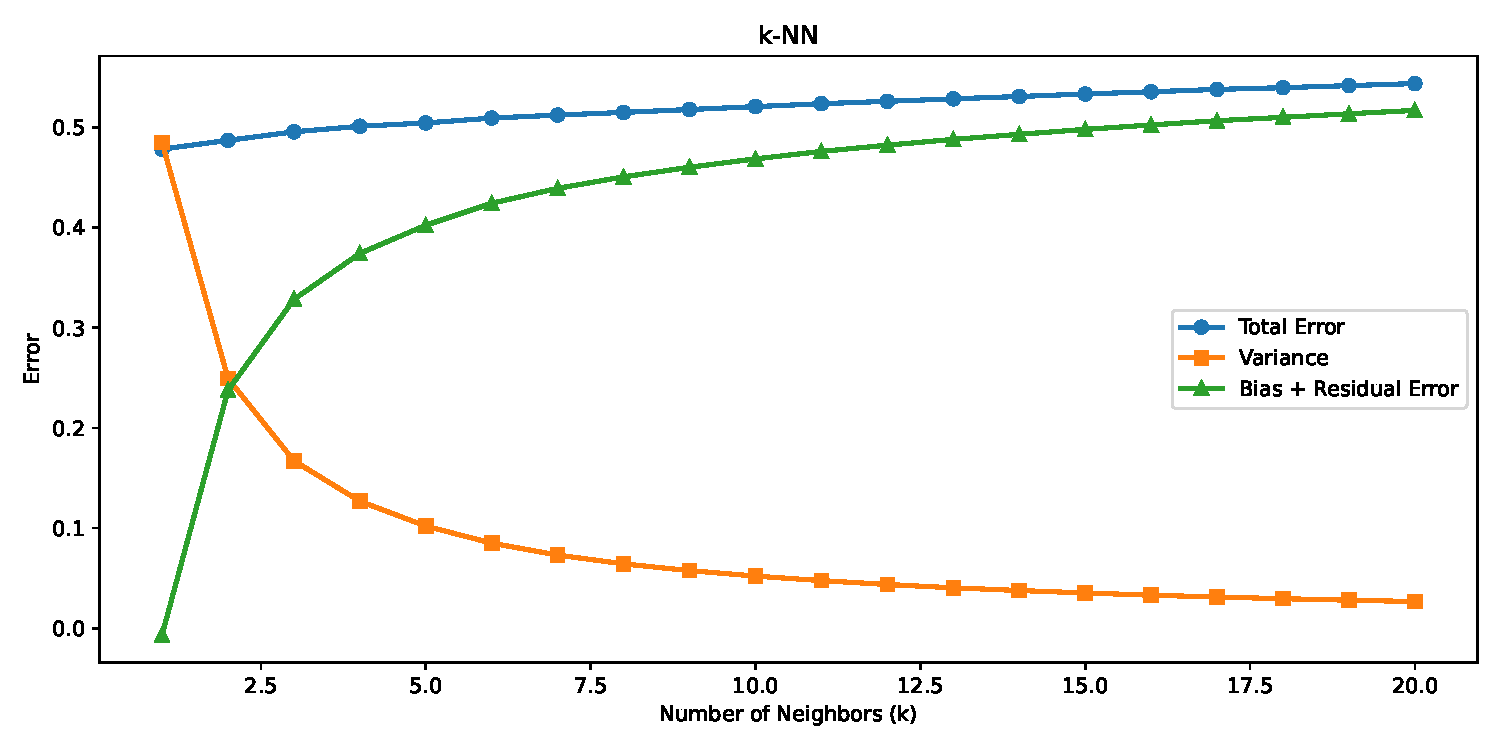
\includegraphics[width=0.8\linewidth]{images/2.3_knn.pdf}
\end{figure}

Discussion:

For k-NN, we varied the number of neighbors \(k\) from 1 to 200. The \textbf{Total Error} decreases sharply as \(k\) increases from small values, indicating improved model performance as more neighbors are incorporated into the predictions. This reflects that averaging over more neighbors reduces the model’s sensitivity to noise and outliers. However, beyond a certain point, the total error stabilizes and then increases. This happens because the model begins to oversmooth as \(k\) becomes too large, effectively averaging over neighbors that may include points from different classes or regions, reducing its ability to make precise predictions for local patterns.

The behavior we observe is consistent with the bias-variance trade-off.
The \textbf{Variance} decreases as \(k\) increases because the model becomes less sensitive to individual data points. For small values of \(k\), the predictions rely heavily on the nearest training points, resulting in high variance. As \(k\) grows, the predictions are averaged over more neighbors, reducing the variability in the predictions and smoothing the model's output. This reduction in variance demonstrates the model's increasing robustness to noise.

The \textbf{Bias + Residual Error} increases with \(k\). When \(k\) is small, the model is highly flexible, capturing fine-grained details in the data, leading to low bias. As \(k\) increases, the model oversmooths the data, failing to capture finer patterns, and the bias grows. The residual error remains constant as it is intrinsic to the data and independent of the model's complexity.

Thus, the optimal k represents a balance between bias and variance, minimizing the total error by achieving the right trade-off between underfitting and overfitting.


\subsubsection{Lasso}

\begin{figure}[H]
    \centering
    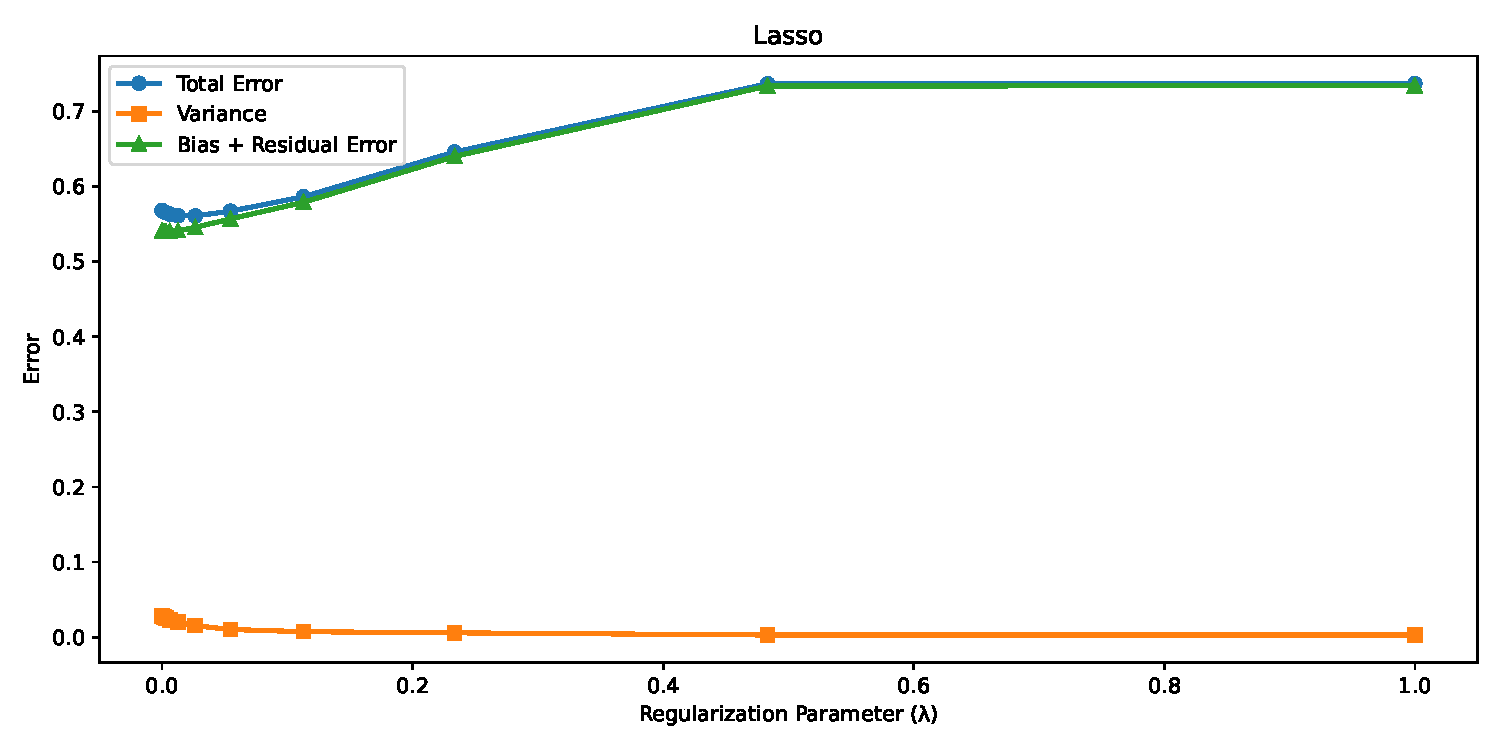
\includegraphics[width=0.8\linewidth]{images/2.3_lasso.pdf}
\end{figure}

Discussion:

For Lasso regression, we varied the regularization parameter \(\lambda\) on a logarithmic scale, ranging from \(10^{-6}\) to \(10^0\). The graph shows the behavior of the total error, variance, and the sum of bias and residual error as \(\lambda\) increases.

As \(\lambda\) increases, the \textbf{Total Error} (blue curve) gradually rises. This behavior indicates that the model becomes too simplistic, leading to underfitting. The increase in \(\lambda\) penalizes the magnitude of the model’s coefficients, forcing them towards zero. While this reduces overfitting, it also limits the model’s flexibility to fit the data, causing it to miss important patterns and increasing the error.

The \textbf{Variance} (orange curve) decreases sharply as \(\lambda\) increases. This is because the regularization term suppresses large coefficients, making the model less sensitive to small fluctuations or noise in the training data. A smaller variance implies that the predictions are more stable across different subsets of the data, reflecting the model's reduced sensitivity to overfitting.

On the other hand, the \textbf{Bias + Residual Error} (green curve) increases with \(\lambda\). As the model is regularized more heavily, it becomes overly simplistic and fails to capture the complexity of the underlying data distribution. This behavior exemplifies the classic \textbf{bias-variance trade-off}: higher regularization reduces variance but increases bias.

The optimal value of \(\lambda\) is in a region where the total error is minimized, balancing the trade-off between bias and variance. At this point, the regularization is sufficient to prevent overfitting while retaining enough model complexity to capture the significant patterns in the data. Beyond this point, further increases in \(\lambda\) lead to diminishing returns, as the model’s ability to represent the underlying data diminishes.


\subsubsection{Regression Tree}

\begin{figure}[H]
    \centering
    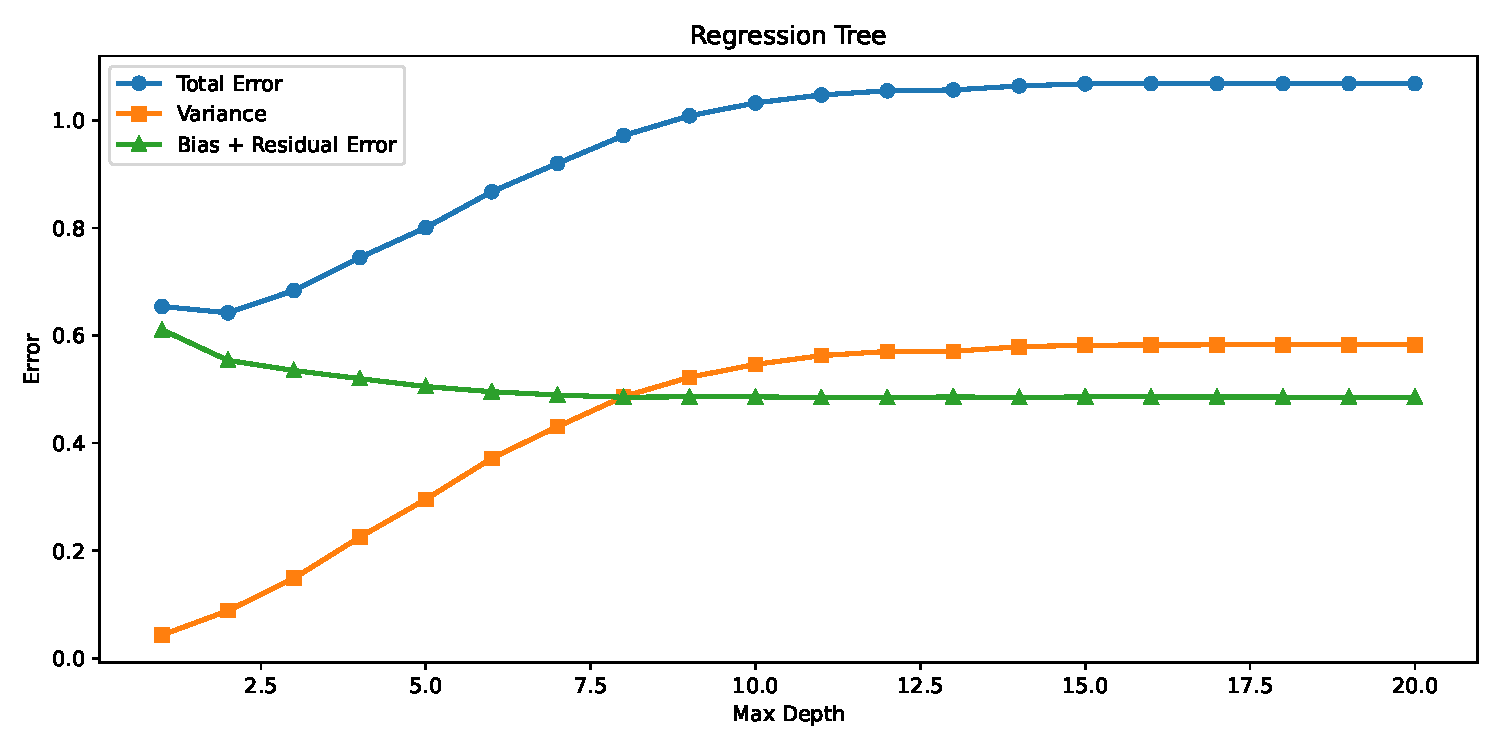
\includegraphics[width=0.8\linewidth]{images/2.3_rt.pdf}
\end{figure}

Discussion:

For Regression Trees, we varied the maximum depth from 1 to 20. Initially, as the depth increases, the \textbf{Total Error} (blue curve) decreases. This indicates that the tree is capturing more complex patterns in the data, improving model performance. However, after reaching an optimal depth, further increasing the depth leads to an increase in total error, as the model starts overfitting the training data. Overfitting occurs because the tree becomes excessively complex and adapts to noise in the data.

The \textbf{Variance} (orange curve) increases with the maximum depth. Deeper trees are more sensitive to the training data, capturing noise and fluctuations, which results in higher variance. This sensitivity causes the model to perform inconsistently across different datasets, reducing its generalization ability.

The \textbf{Bias + Residual Error} (green curve) decreases as the depth increases. Shallow trees have high bias because they are too simple to capture the underlying relationships in the data, leading to systematic errors. As the tree becomes more flexible with increased depth, it models more complex relationships and reduces bias. However, this comes at the cost of increased variance.

This behavior follows the classic \textbf{bias-variance trade-off}: shallow trees exhibit high bias but low variance (underfitting), while deeper trees show low bias but high variance (overfitting). The optimal depth achieves a balance, capturing enough complexity to reduce bias while controlling the variance.




    
%% Question 2.4: For the same three methods, show the impact of the learning sample size on bias and 
% variance.

\subsection{}

\subsubsection{kNN - k=5}

\begin{figure}[H]
    \centering
    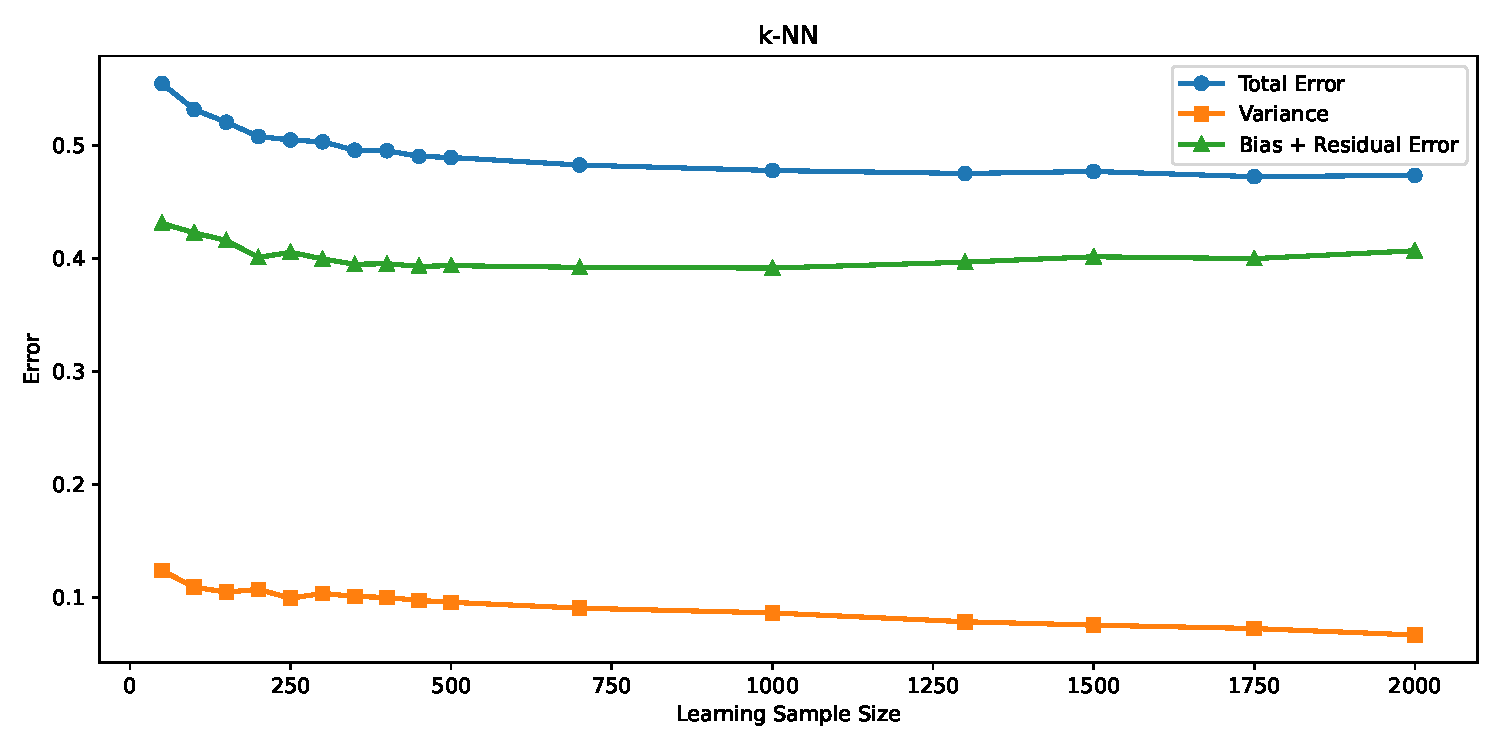
\includegraphics[width=0.8\linewidth]{images/2.4_knn.pdf}
\end{figure}

Discussion:  
For \(k\)-NN, we fixed the number of neighbors to 5 and varied the learning sample size. The plot shows that as the learning sample size increases, the \textbf{Total Error} decreases, indicating improved model performance with more data. The \textbf{Variance} also decreases with increasing sample size, as the model becomes more stable and less sensitive to individual data points. We can also observe the \textbf{Bias} decreasing as the sample size grows. 

This occurs because a larger sample size provides more representative data points for the model to learn from, reducing the likelihood of overfitting specific regions of the data. Additionally, as the sample size increases, the effective complexity of the model increases, as it gains access to a richer set of information to make more precise predictions. This reduces the bias caused by an insufficiently diverse training set.

Larger datasets enable \(k\)-NN to approximate the true underlying data distribution more effectively, improving both generalization and accuracy. However, as the sample size continues to grow, the rate of improvement in model performance diminishes. This is because the model reaches a point where it has effectively captured the underlying data distribution, and further increases in the sample size provide minimal additional benefit. At this stage, the residual error, which represents the irreducible noise in the data, becomes the dominant factor in the total error.

In summary, increasing the sample size improves the model’s ability to generalize by lowering both variance and bias. However, past a certain point, the model's performance stop improving as it approaches its theoretical limit (constrained by the residual error).


\subsubsection{Lasso - $\lambda$ = 0.01 }

\begin{figure}[H]
    \centering
    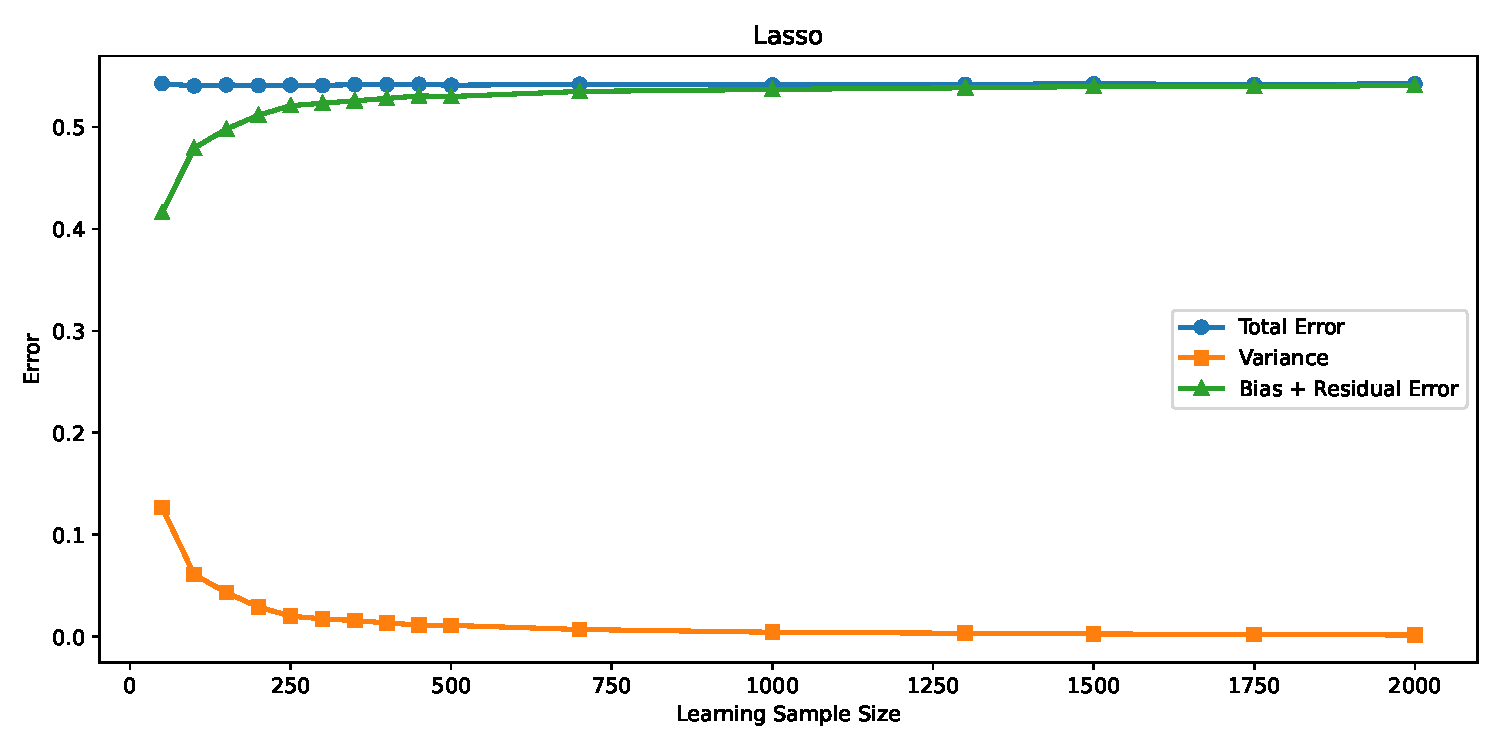
\includegraphics[width=0.8\linewidth]{images/2.4_lasso.pdf}
\end{figure}

Discussion:  
For Lasso, we fixed the regularization parameter to 0.01 and varied the learning sample size. The plot shows that as the learning sample size increases, the \textbf{Total Error} decreases, indicating improved model performance with more data. The \textbf{Variance} decreases with increasing sample size as well, as the model becomes more stable and less sensitive to noise in the training set. The \textbf{Bias} remains relatively constant, suggesting that the ability of Lasso to capture the underlying patterns does not change significantly with more data, which is consistent with the fixed regularization parameter.

As the sample size increases, the \textbf{Variance} decreases due to a more robust coefficient estimation. With larger datasets, the model can better distinguish signal from noise, leading to more stable predictions. However, the \textbf{Bias} remains largely unaffected because the regularization strength, determined by the fixed \(\lambda = 0.01\), controls the model's complexity. This fixed regularization parameter constrains the model by penalizing large coefficients, effectively limiting the number of features it can use to make predictions. Even with a larger sample size, the regularization term prevents the model from increasing its complexity, maintaining the same level of approximation for the underlying data distribution. 

This behavior occurs because the regularization term explicitly controls the model's capacity to fit the data by forcing many coefficients towards zero or small values. As a result, regardless of how much data is added, the bias, which depends on the model's flexibility, does not change. The model remains constrained by the fixed \(\lambda\).

This illustrates that the performance of Lasso is more dependent on the choice of regularization parameter than on the sample size. While a larger sample size helps in reducing variance, the bias is primarily controlled by the regularization term, which dictates how much complexity the model can incorporate. In summary, the total error decreases with increasing sample size due to the reduction in variance, but the bias remains constant, reflecting the model's fixed complexity as determined by the regularization parameter.



\subsubsection{Regression Trees - Fixed Depth}

\begin{figure}[H]
    \centering
    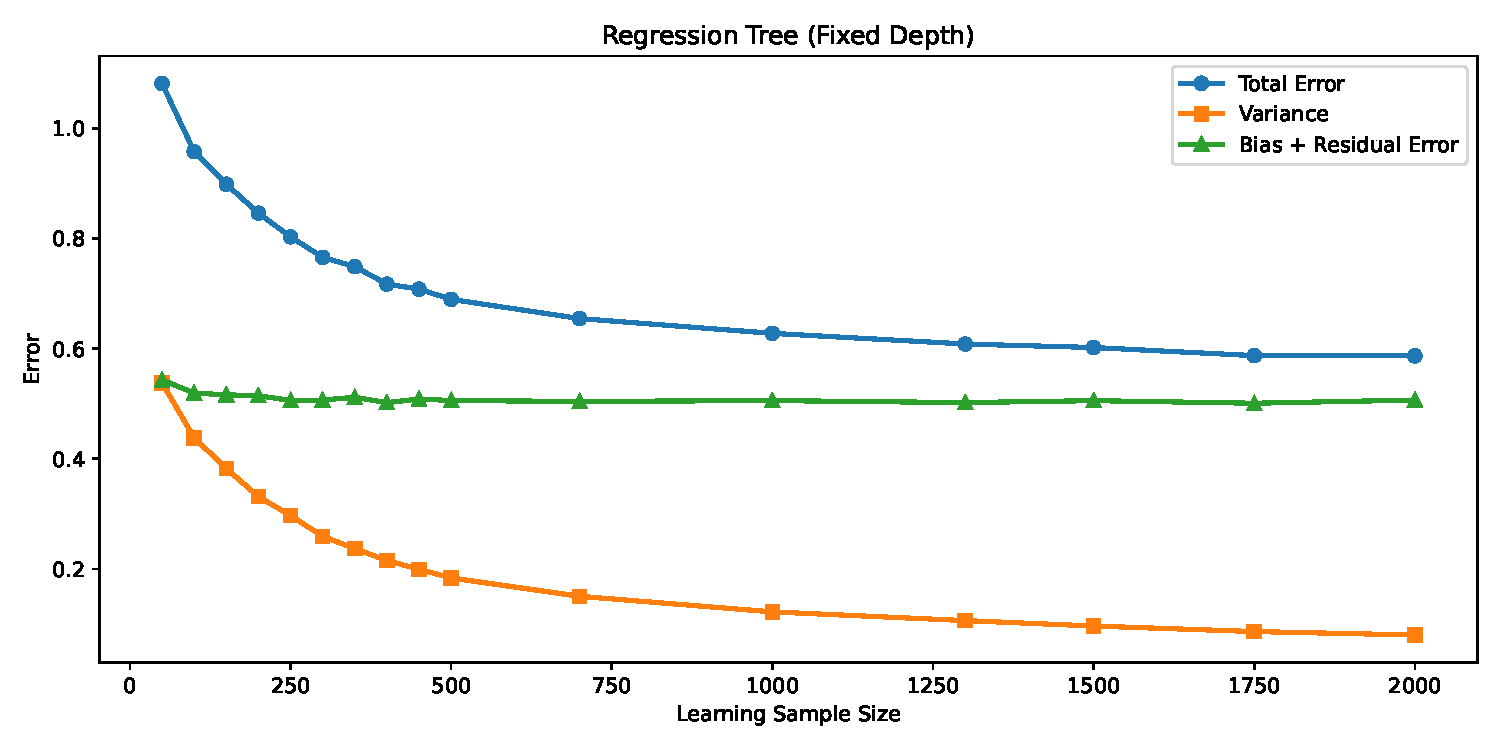
\includegraphics[width=0.8\linewidth]{images/2.4_rt_fixed.pdf}
\end{figure}

Discussion:  
For the regression tree with fixed depth, we set the maximum depth to 5 and varied the learning sample size. The plot shows that as the learning sample size increases, the \textbf{Total Error} decreases, indicating improved model performance with more data. The \textbf{Variance} decreases as well, similar to the behavior observed in Lasso and \(k\)-NN, as the model becomes more stable and less sensitive to individual data points. The \textbf{Bias} remains constant, reflecting the fixed complexity of the tree, which cannot adapt to the larger dataset, like with the regularization parameter in Lasso.

Increasing the sample size reduces \textbf{Variance}, as the model benefits from a more representative dataset, making it more stable and less prone to overfitting. However, the \textbf{Bias} remains unaffected because the tree's depth is fixed, restricting its ability to capture more complex patterns regardless of the sample size.

In summary, as in \(k\)-NN and Lasso, increasing the sample size reduces variance, but the bias stays constant due to the fixed model complexity. The total error decreases because of this reduction in variance, but the bias remains constant, as the model's capacity to learn complex relationships is limited by the fixed depth.


\subsubsection{Regression Tree - Full}

\begin{figure}[H]
    \centering
    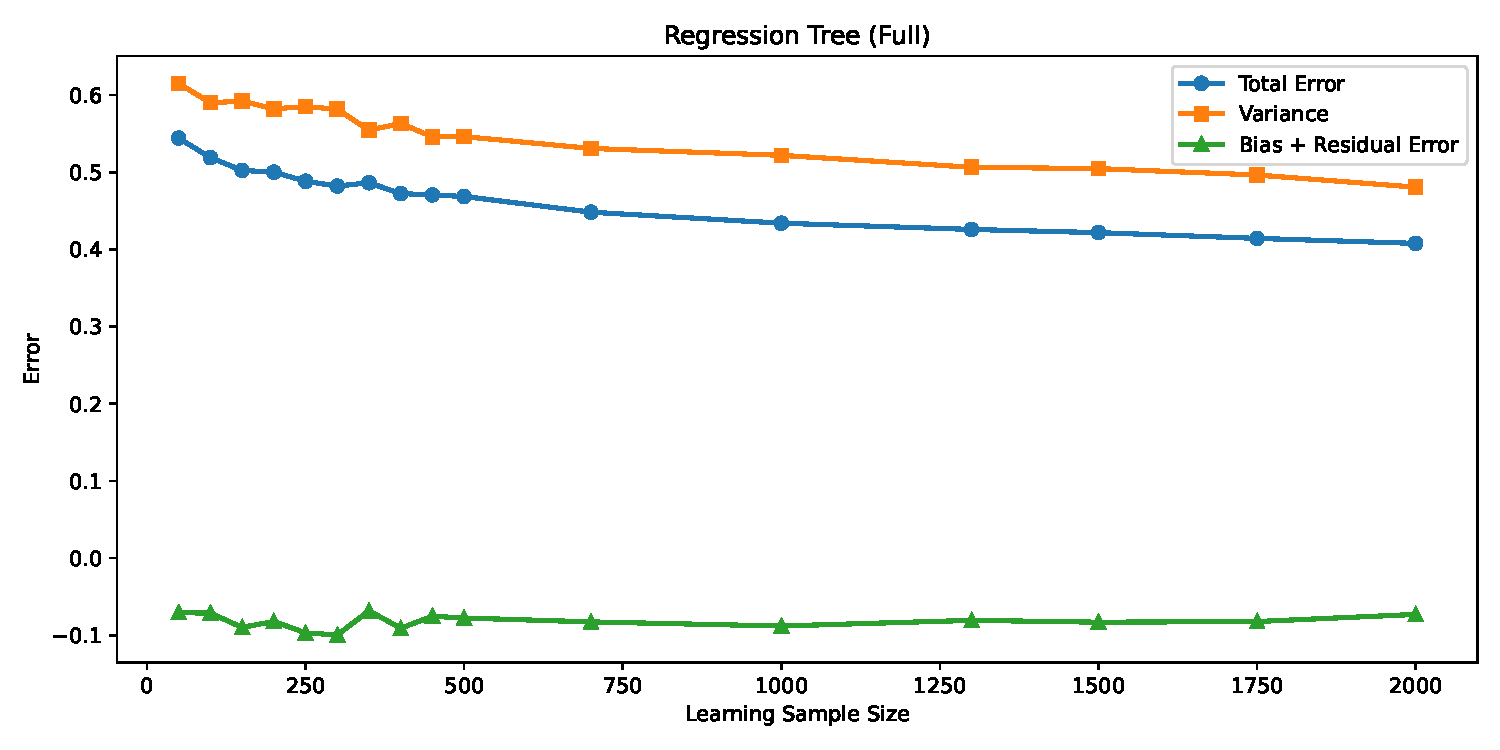
\includegraphics[width=0.8\linewidth]{images/2.4_rt_full.pdf}
\end{figure}

Discussion:  
For the regression tree with full depth, we allowed the tree to grow without any depth restriction and varied the learning sample size. The plot shows that as the learning sample size increases, the \textbf{Total Error} decreases, indicating improved model performance with more data. The \textbf{Variance} decreases with increasing sample size, as the model becomes more stable and less sensitive to individual data points, similar to the behavior observed in \(k\)-NN and Lasso.

The \textbf{Bias} decreases as the sample size grows. With infinite depth, the tree can perfectly fit the data by capturing all patterns, including the smallest ones, thus reducing bias. This is because a deeper tree has more flexibility to model the data, fitting the underlying relationships more accurately. As a result, the model can better approximate the true data distribution, reducing the bias. In contrast to a shallow tree, which is limited in its capacity to model complexity, the tree with full depth has a lower bias, especially when provided with more data.

However, the tree with full depth has an higher variance, especially when the sample size is small, as it tends to overfit the data. As the sample size increases, overfitting is mitigated, and the model's variance reduces.

In summary, increasing the sample size in a fully grown regression tree reduces both variance and bias, improving the model’s performance.





    %% Question 2.5: Two so-called ensemble methods to address variance and bias are bagging 
    % ("bootstrap aggregating") and boosting. 
\subsection{}

\subsubsection{Bagging}
\begin{figure}[H]
    \centering
    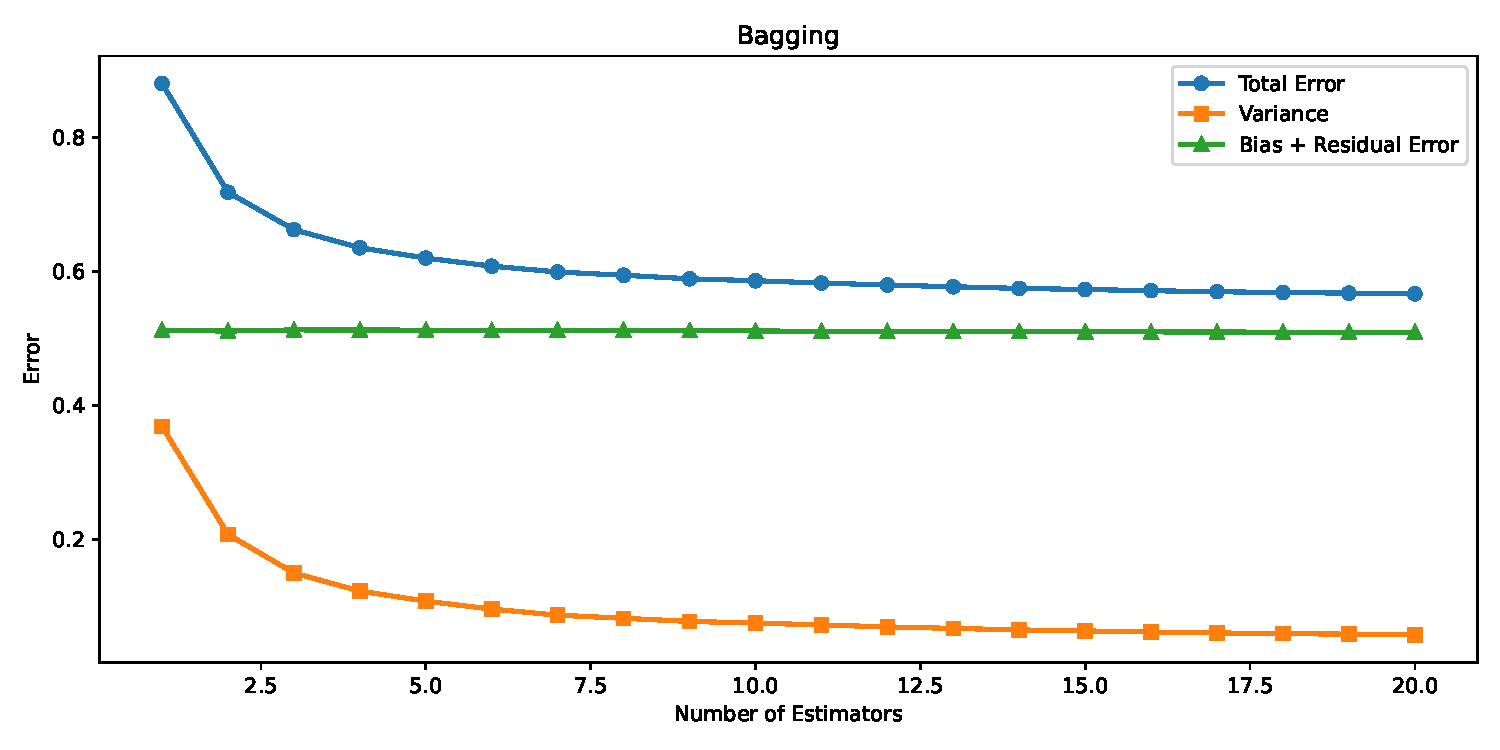
\includegraphics[width=0.8\linewidth]{images/2.5_bagging.pdf}
\end{figure}

Discussion:
        

\subsubsection{Boosting}
\begin{figure}[H]
    \centering
    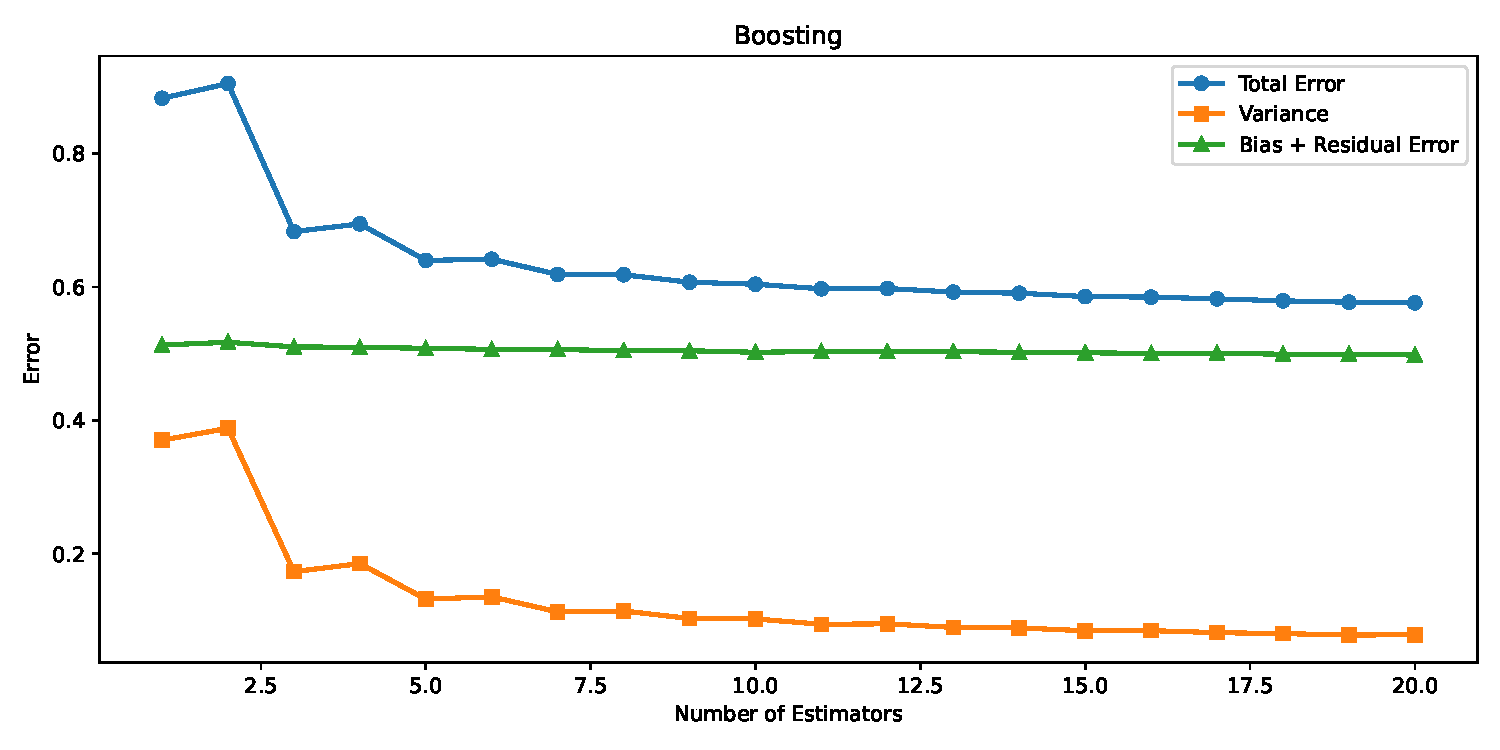
\includegraphics[width=0.8\linewidth]{images/2.5_boosting.pdf}
\end{figure}

Discussion:

\subsubsection{Complexity influence}

Below are the plots of the total error, bias (bias squared + residual error), and variance of the result using the bagging method.

\begin{figure}[H]
    \centering 
    \begin{minipage}{0.33\textwidth}
        \centering
        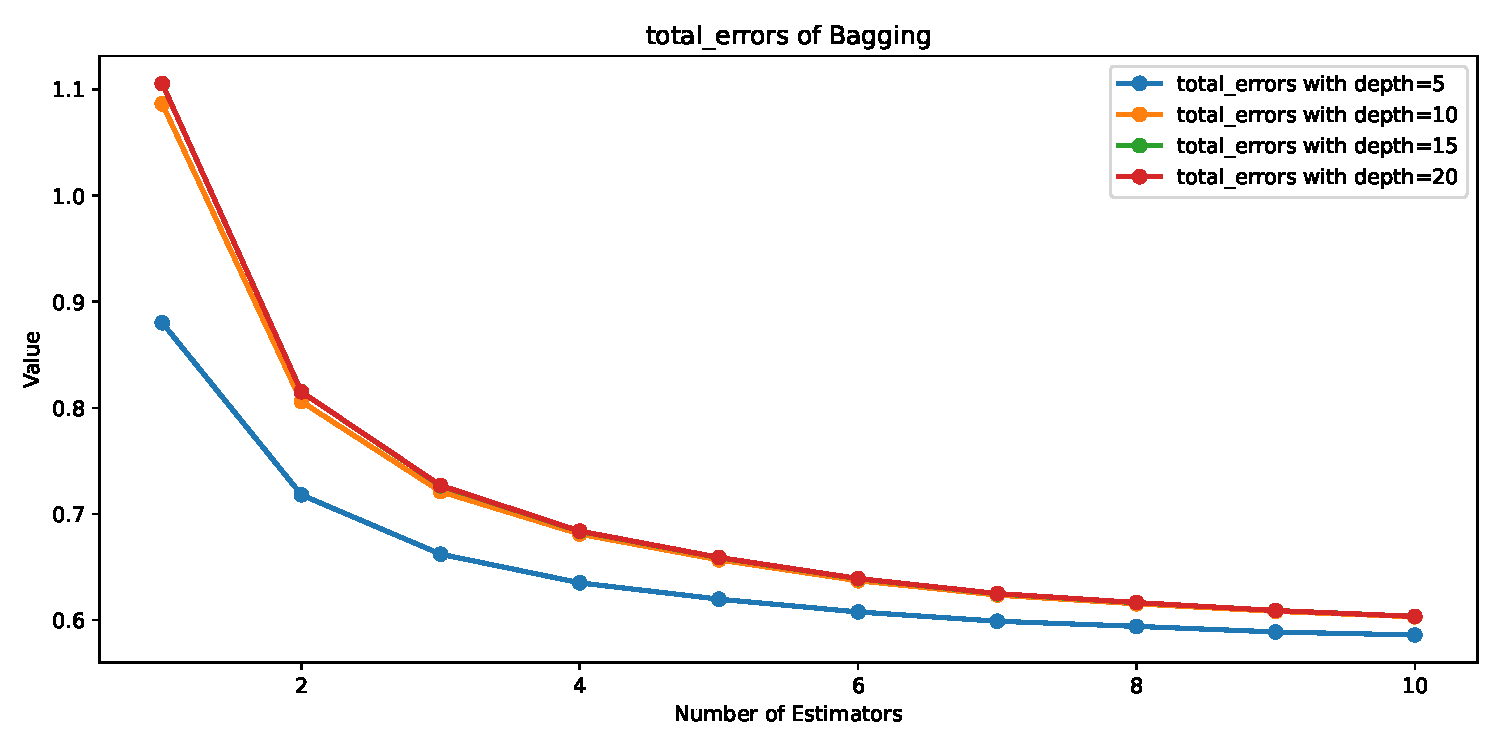
\includegraphics[width=\linewidth]{images/2.5_total_error_bagging.pdf}
        \caption{Evolution of total error}
    \end{minipage}%
    \begin{minipage}{0.33\textwidth}
        \centering
        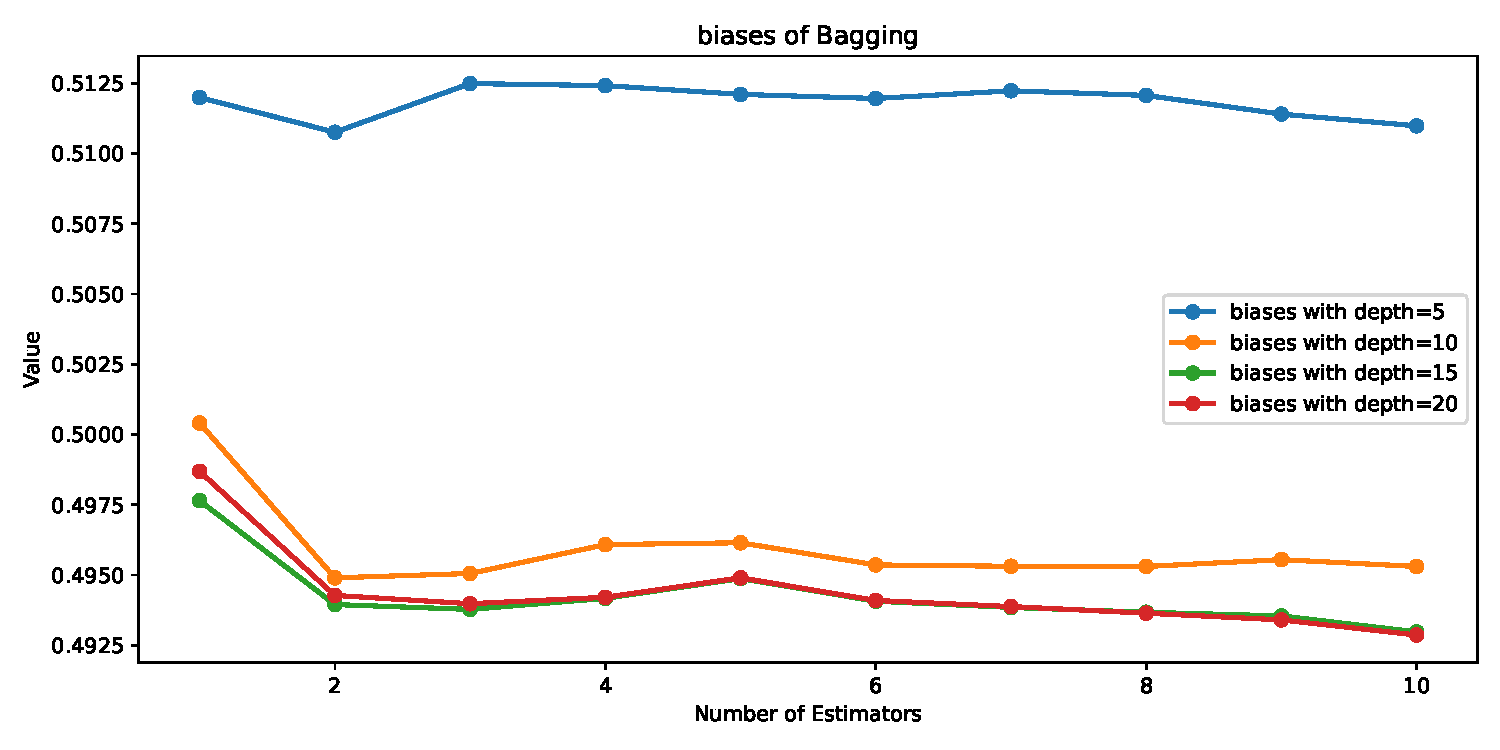
\includegraphics[width=\linewidth]{images/2.5_bias_bagging.pdf}
        \caption{Evolution of bias}
    \end{minipage}%
    \begin{minipage}{0.33\textwidth}
        \centering
        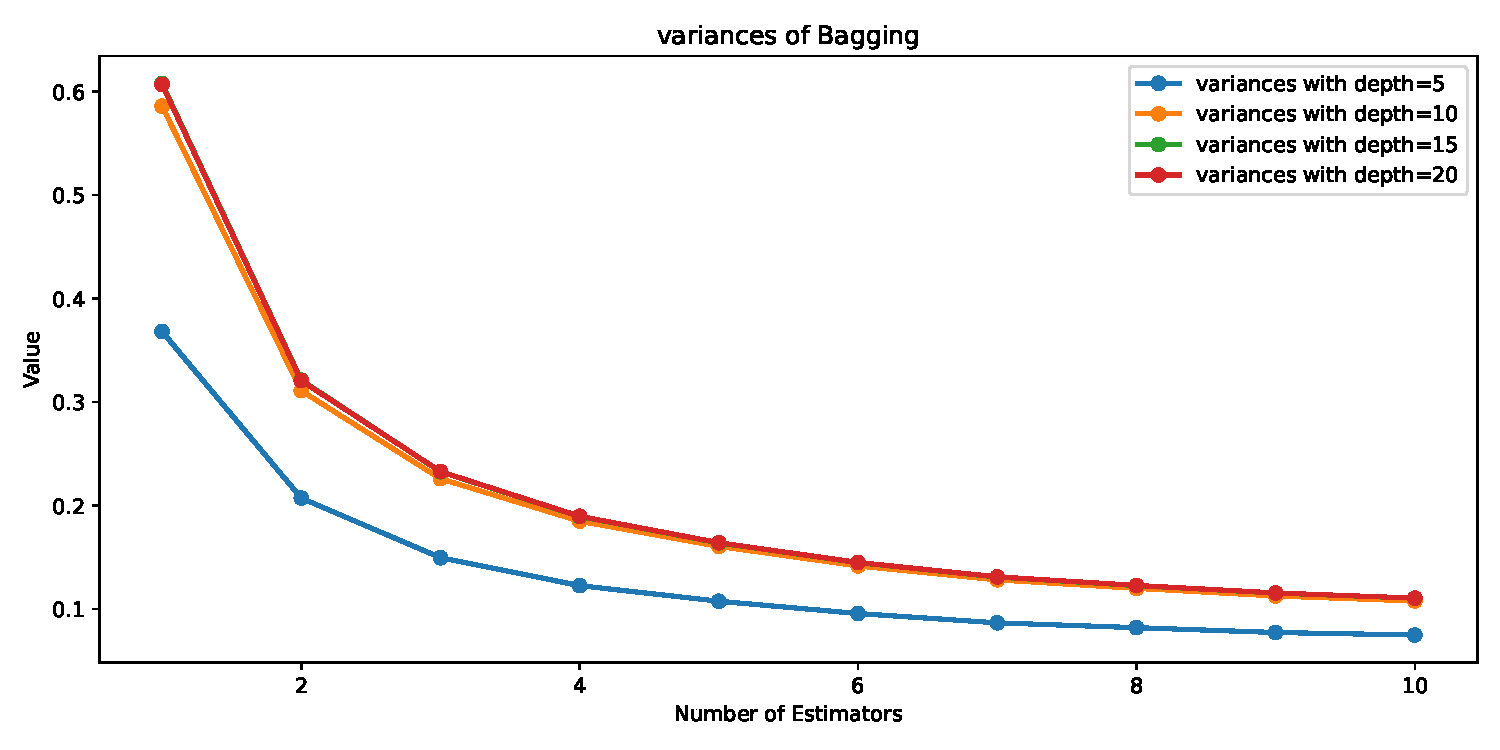
\includegraphics[width=\linewidth]{images/2.5_var_bagging.pdf}
        \caption{Evolution of var}
    \end{minipage}
    \caption{Evolution of bagging results based on the max depth.}
\end{figure}

Discussion:


Below are the plots of the total error, bias (bias squared + residual error), and variance of the result using the boosting method.

\begin{figure}[H]
    \centering 
    \begin{minipage}{0.33\textwidth}
        \centering
        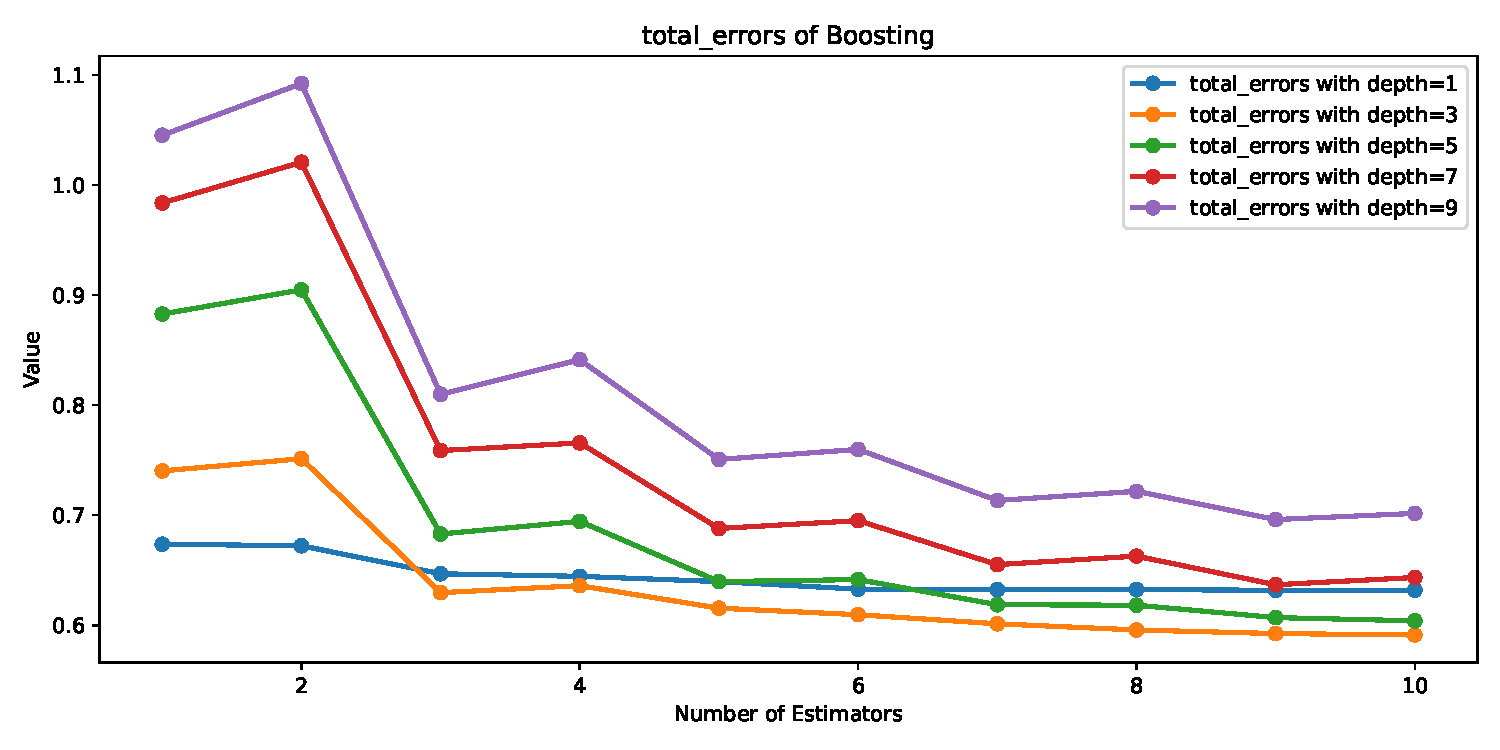
\includegraphics[width=\linewidth]{images/2.5_total_error_boosting.pdf}
        \caption{Evolution of total error}
    \end{minipage}%
    \begin{minipage}{0.33\textwidth}
        \centering
        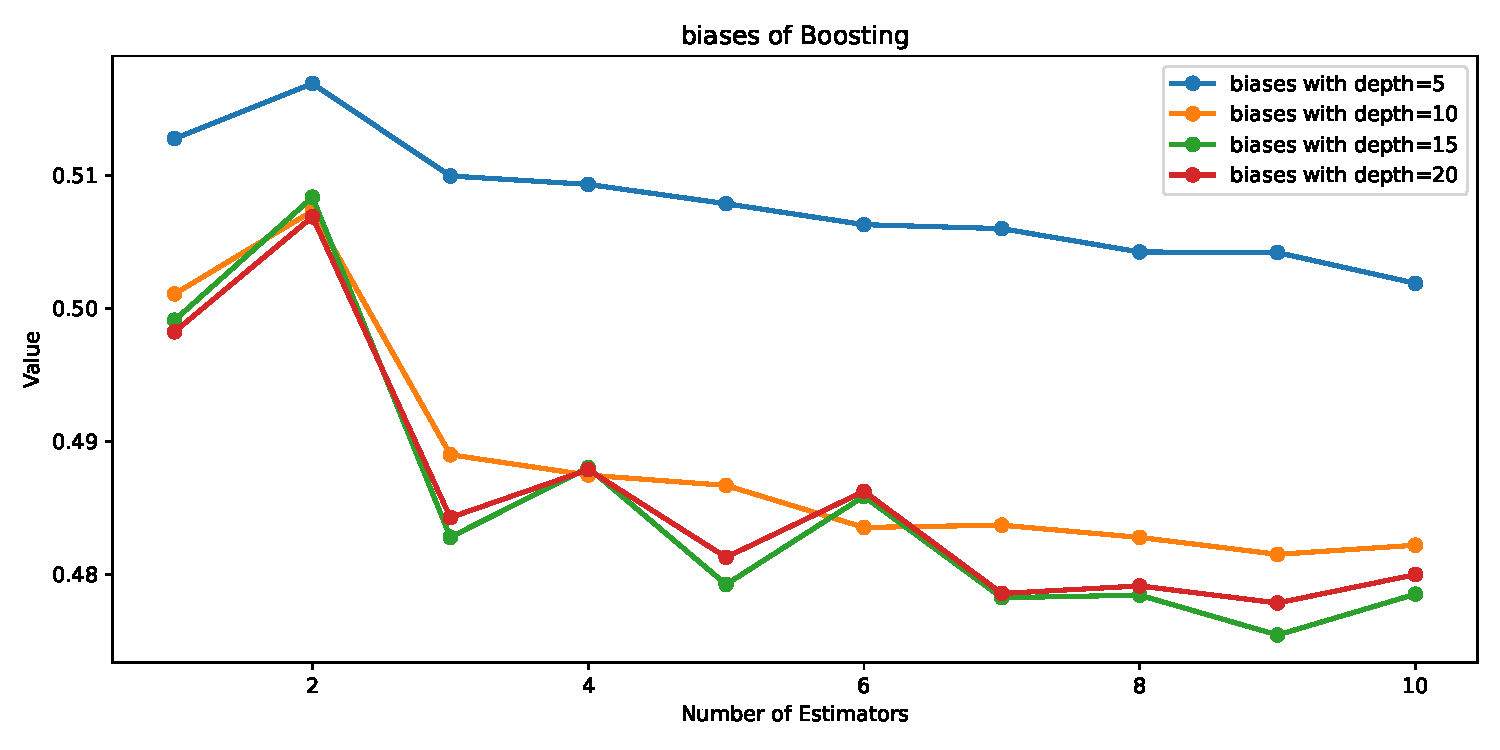
\includegraphics[width=\linewidth]{images/2.5_bias_boosting.pdf}
        \caption{Evolution of bias}
    \end{minipage}%
    \begin{minipage}{0.33\textwidth}
        \centering
        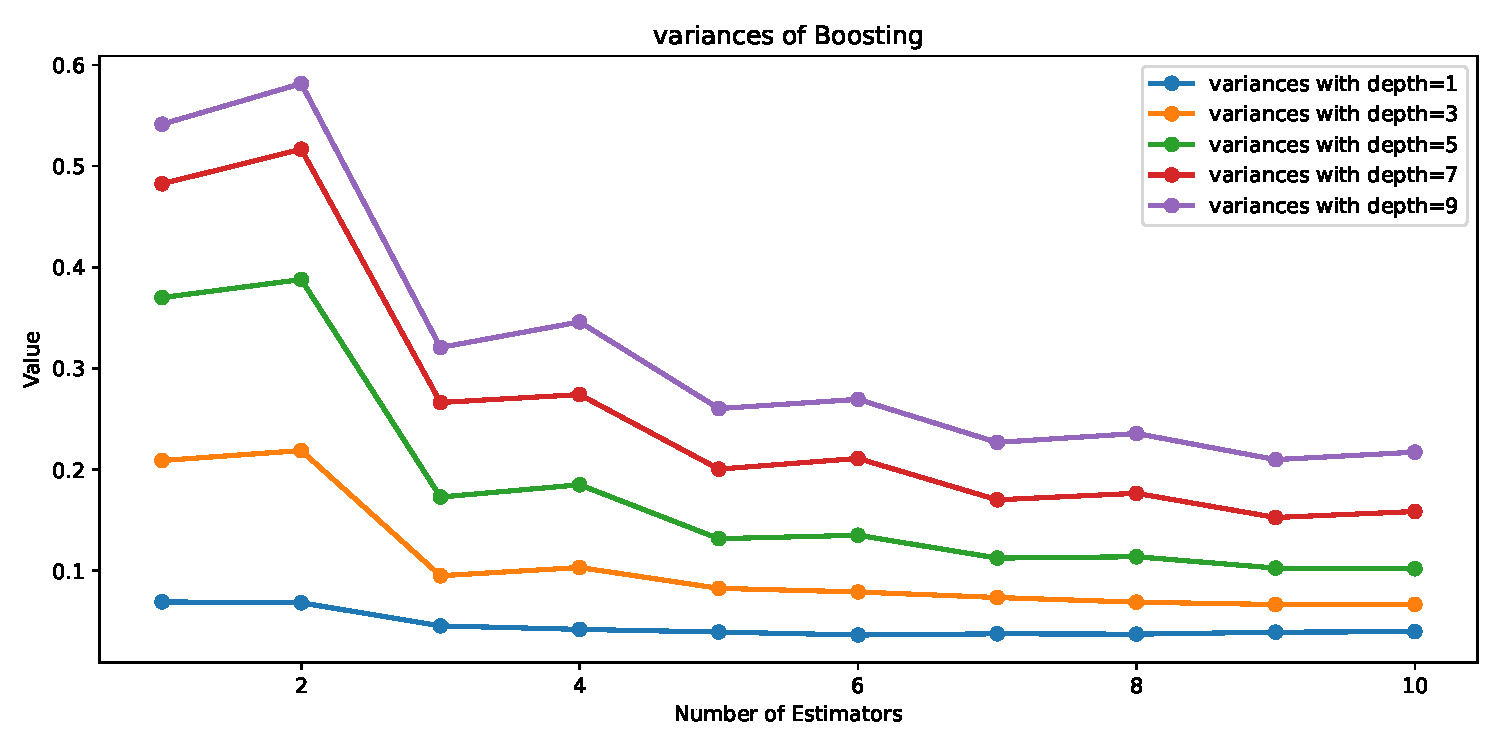
\includegraphics[width=\linewidth]{images/2.5_var_boosting.pdf}
        \caption{Evolution of var}
    \end{minipage}
    \caption{Evolution of boosting results based on the max depth.}
\end{figure}

Discussion:
The boosting should have a lower bias but it doesn't doesn't decrease significantly and the base value is as high as using other models. Since the bias doesn't decrease as it should, using boosting doesn't give good results in this case.

\end{document}